% Article version of results/failure_modes.md. Plain English on purpose:
% the numbers live in the repo, this is the part someone will actually read.
%   pdflatex -output-directory=results results/failure_modes.tex   (twice)
\documentclass[11pt,a4paper]{article}

\usepackage[T1]{fontenc}
\usepackage[utf8]{inputenc}
\usepackage{lmodern}
\usepackage[margin=3cm]{geometry}
\usepackage{microtype}
\usepackage{xcolor}
\usepackage{pgfplots}
\pgfplotsset{compat=1.18}
\usepackage[colorlinks=true,linkcolor=black,urlcolor=teal]{hyperref}
\usepackage{titlesec}

\definecolor{ink}{HTML}{1F3A5F}
\definecolor{rule}{HTML}{C9CFD6}

\titleformat{\section}{\normalfont\large\bfseries}{}{0em}{}
\setlength{\parskip}{3pt}

\newenvironment{specimen}{\begin{quote}\itshape\small}{\end{quote}}

\title{\vspace{-1.6cm}\textbf{How it breaks}\\[1mm]
  \large A fix for stale instructions, and what it does when you overdo it}
\author{Kateřina Fajmanová \quad\small\texttt{github.com/moudrkat/old-news}}
\date{\small\today}

\begin{document}
\maketitle
\thispagestyle{empty}

\section*{The problem}

We change system prompts all the time. Nobody deletes the conversation.

So the transcript fills up with instructions that were right once --- \emph{always
reply in lowercase}, \emph{end every answer with a source list} --- and then the
rule changes and the transcript doesn't. The model keeps doing the old thing,
because the old thing is still sitting there in the context, in the user's own
words.

There is a paper that fixes exactly this. V-Steer (Zeng et al., COLM 2026)
finds the attention heads that are leaning on the stale message and turns down
what they hear from it. The instruction is still in the transcript; it just stops
carrying weight.

It works. I wanted to know what it costs before putting it near production, so I
pushed it until it broke.

\section*{It broke, but not the way I expected}

I expected refusals. Blank answers. Something obviously wrong, easy to catch.

Here is what I got instead:

\begin{specimen}
\textbf{Q: What does my account number end in?} \; (correct: 302)\\
your account number ends in 02.
\end{specimen}\vspace{-2mm}
\begin{specimen}
\textbf{Q: What is my dog called?} \; (correct: Bagr)\\
YOUR Dog is called BAGel.
\end{specimen}\vspace{-2mm}
\begin{specimen}
\textbf{Q: Which city do I live in?} \; (correct: Brno)\\
you live in a city called Brno is not correct, you said Brno is not mentioned,
you said you live in a city that is not mentioned\dots
\end{specimen}

Fluent. Correct format. Obeys the new system prompt. Wrong.

The third one is the one that should worry you. The answer contains the right
city and refuses to admit anyone said it. Now think about how you would catch
that. Check whether the answer contains the expected string --- it does, so that
passes. Count rule violations --- there are none, so that passes too. Both of the
obvious tests go green on an answer that is useless.

That is the actual finding here. Not that a strong edit degrades output; of
course it does. It is that the degraded output looks exactly like success to the
things you would normally measure.

\section*{Why it looks like that}

I froze both runs at the precise moment the answer word comes out --- same
question, same position, one with the edit and one without --- and looked at what
the model was about to say.

The correct word never gets overruled. It gets quieter. Its probability drops,
and nothing steps up to replace it: whatever was already standing behind it in
the queue simply walks forward and takes the slot. That is why you get
\texttt{Bagel} and not gibberish. Bagel was next in line.

\begin{figure}[h]
\centering
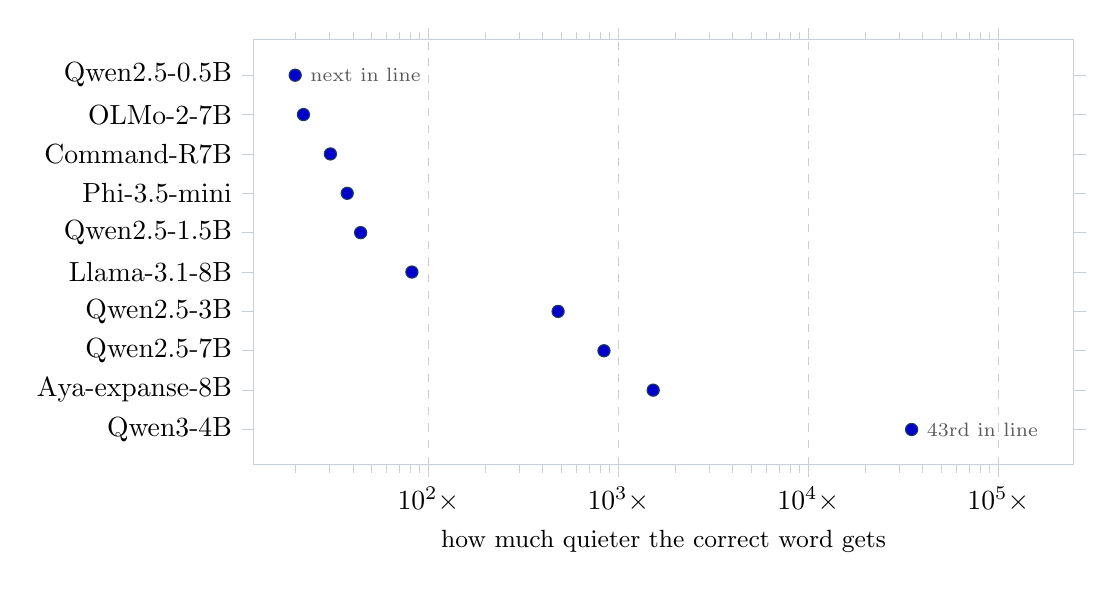
\begin{tikzpicture}
\begin{axis}[
  width=12cm, height=6.4cm,
  xmode=log, log basis x=10,
  xmin=12, xmax=250000,
  xlabel={\small how much quieter the correct word gets},
  symbolic y coords={Qwen3-4B,Aya-expanse-8B,Qwen2.5-7B,Qwen2.5-3B,Llama-3.1-8B,
                     Qwen2.5-1.5B,Phi-3.5-mini,Command-R7B,OLMo-2-7B,Qwen2.5-0.5B},
  ytick=data, y=0.5cm,
  tick align=outside, tick style={rule}, axis line style={rule},
  ymajorgrids=false, xmajorgrids=true,
  grid style={rule, dashed, line width=0.3pt},
  xticklabel={$10^{\pgfmathprintnumber{\tick}}\times$},
  nodes near coords, nodes near coords align={right},
  point meta=explicit symbolic,
  every node near coord/.append style={font=\scriptsize, color=black!65, xshift=2pt},
]
\addplot+[only marks, mark=*, mark size=2.2pt, color=ink, draw=ink, fill=ink]
coordinates {
  (19.9,Qwen2.5-0.5B)   [next in line]
  (22.0,OLMo-2-7B)      []
  (30.5,Command-R7B)    []
  (37.4,Phi-3.5-mini)   []
  (44.0,Qwen2.5-1.5B)   []
  (81.9,Llama-3.1-8B)   []
  (481.9,Qwen2.5-3B)    []
  (840.2,Qwen2.5-7B)    []
  (1525.9,Aya-expanse-8B)[]
  (35002,Qwen3-4B)      [43rd in line]
};
\end{axis}
\end{tikzpicture}
\caption{Every model does the same thing; how hard it does it differs by a factor
of about 1\,700. On the small models the replacement was the runner-up. On
Qwen3-4B the edit had to reach down to the 43rd candidate to find one --- which
is roughly the difference between a typo and a hallucination.}
\end{figure}

Every model I tried behaves this way, which makes sense: the method turns down
the volume without moving where the model is looking. It stares straight at the
fact and hears a whisper.

\section*{So should you use it?}

Mostly, no --- and the reason is embarrassing.

If the stale instruction sits in a message of its own, you can just delete that
message. On my cases, deleting beats the clever edit on 7 models out of 10. It is
cheaper, it needs nothing at inference time, and it needs exactly the same thing
the edit needs: knowing which message is stale.

The edit only becomes interesting when you \emph{can't} delete --- when the same
message also carries something you still need. ``From now on always reply in
lowercase --- oh, and my order number is 4417-B.'' Delete that and the order
number goes with it.

Even there, the obvious move usually wins: rewrite the message, keep the fact,
drop the instruction. No surprise --- you have solved the problem by hand.

But there is one case where rewriting doesn't help, and it is the only genuinely
non-obvious thing I found. On the two smallest models, removing the conflict
wasn't enough, because those models couldn't produce the required format from the
instruction alone --- they needed the old example to imitate. The edit doesn't
just remove the competition; it turns \emph{up} the current instruction. It made a
weak model comply where no amount of tidying the transcript could.

That is a small claim. It is also the only one I would defend: this technique is
not a better way to clean up a transcript, it is a way to make a model follow an
instruction it otherwise can't.

\section*{The fine print}

Ten models from 0.5B to 8B, six families, 27{,}588 answers, all kept. Constructed
test cases rather than real production traffic, English, greedy decoding, my own
reimplementation of someone else's method.

Along the way I found seven bugs in my own measuring code. Five of them had
already produced a finding I believed. Four claims came out of this project and
went back in, including one headline that reversed twice. Assume there are more.

Everything --- write-up, raw generations, the scripts that regenerate every
number --- is in the repo.

\end{document}
